{\Large Diagonalisation} \\
\marginnote[0cm]{Le texte suivant est extrait de \cite{oraux_x_ens_2} p. 169.}
\begin{marginfigure}[1cm]
    \centering
    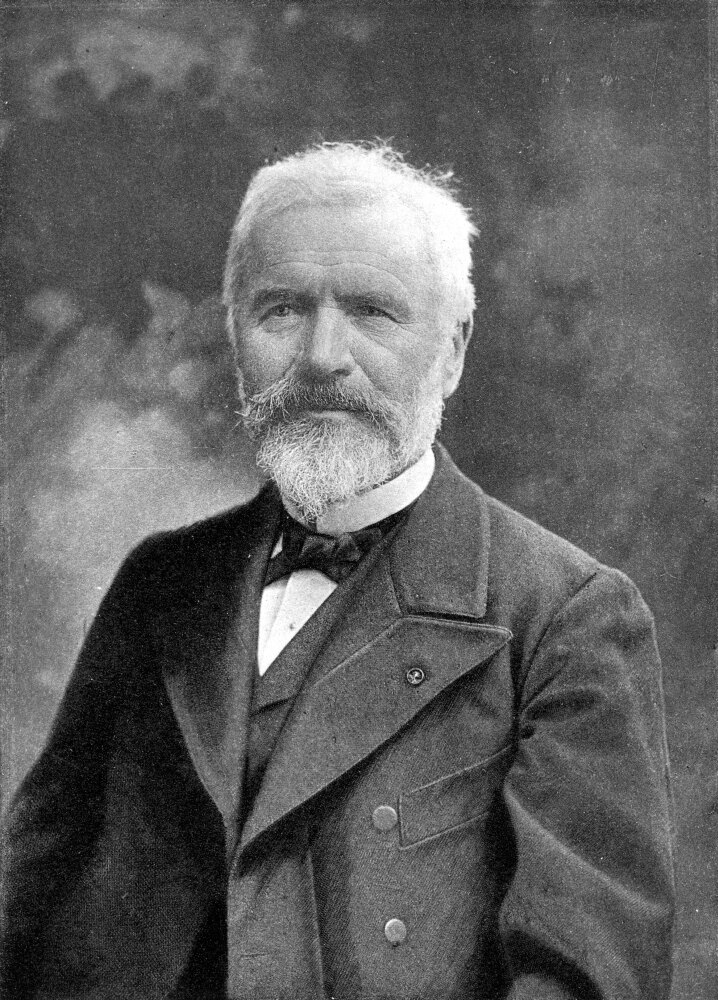
\includegraphics[width=5cm]{images/camille_jordan.jpg}
    \caption*{\centering Camille \textsc{Jordan} (1838 - 1922)}
\end{marginfigure}
\textsl{On doit à Camille \textsc{Jordan} de nombreux résultats sur la réduction des endomorphismes qu'il découvre notamment à travers l'étude des groupes. \\
Le problème fondamental de la réduction est bien celui de caractériser les classes de similitude de l'algèbre $\Endo(E)$ où $E$ est un $\K$-espace vectoriel de dimension finie ou, ce qui revient au même, les classes de similitudes de l'agèbre $\M_n(\K)$. La recherche d'une matrice la plus simple possible pour représenter un endomorphisme donné vise de multiples buts: calculer les puissances successives de cet endomorphisme, son commutant, résoudre des systèmes différentiels linéaires... Une idée naturelle pour essayer de \say{ réduire } l'étude d'un endomorphisme $u$ donné à des choses plus simples consiste à essayer de décomposer l'espace vectoriel $E$ en une somme directe de sous-espaces non triviaux stables par $u$. Cela n'est évidemment pas toujours possible. Les sous-espaces stables les plus simples sont ceux sur lesquels $u$ coïncide avec une homothétie. On est ainsi naturellement amené à la notion de valeur propre. Si $\lambda$ est un scalaire, on s'intéresse donc au sous-espace $E_\lambda = \Ker(u - \lambda \Id_E)$ appelé sous-espace propre pour la valeur propre $\lambda$ lorsque celui-ci n'est pas nul. Le théorème de décomposition des noyaux nous assure que les différents sous-espaces propres d'un endomorphisme sont en somme directe. Le cas où la somme remplit tout l'espace $E$ mène à la notion d'endomorphisme diagonalisable: un tel endomorphisme peut être représenté par une matrice diagonale (il suffit de prendre une base formée de vecteurs propres). Pour les endomorphismes diagonalisables il est alors très facile de répondre à la question initiale de savoir quand ils sont semblables: il faut et suffit qu'ils aient les mêmes valeurs propres et que les espaces propres associés aient la même dimension. Il est aussi facile, en se ramenant à une matrice diagonale, de calculer les puissances d'un tel endomorphisme, son exponentielle (si on travaille sur un sous-corps de $\C$), son commutant...}